\documentclass[aspectratio=169]{beamer}

\usepackage{amsmath}
\usepackage{tikz}
\usepackage{pgfplots}
\usepackage{adjustbox}
\usepackage{hyperref}
\usepackage{booktabs}

\pgfplotsset{compat=1.18}
\usetikzlibrary{positioning, arrows.meta}

\usetheme{Madrid}

\title{Santa's Workshop Tour Optimization\\Final Presentation}
\author{Deniz Günes, Simão Ribeiro, Sara Ribeiro}

\begin{document}

\frame{\titlepage}

\begin{frame}{1. Problem Definition}
\textbf{Goal:}
\begin{itemize}
    \item Assign each of the 5,000 families to one of the 100 days preceding Christmas, minimizing the total cost.
\end{itemize}

\textbf{Objective Function:}
\[
f(S) = \text{Preference Cost} + \text{Accounting Penalty}
\]

\textbf{Constraints:}
\begin{itemize}
    \item \textbf{Hard:} Daily occupancy must be between 125 and 300 people.
    \item \textbf{Soft:} Family preferences (10 ranked choices per family).
\end{itemize}
\end{frame}

\begin{frame}{2. Related Work}
\textbf{Sources Explored:}
\begin{itemize}
    \item Kaggle Santa Workshop 2019 Leaderboard Solutions.
    \item Metaheuristics literature (Gendreau \& Potvin).
\end{itemize}

\textbf{Common Techniques Identified:}
\begin{itemize}
    \item \textbf{Simulated Annealing:} Widely used for its ability to escape local optima via probabilistic moves.
    \item \textbf{Large Neighborhood Search:} Effective for highly constrained scheduling problems.
\end{itemize}
\end{frame}

\begin{frame}{3. Problem Formulation}
\textbf{Solution Representation:}
\begin{itemize}
    \item A vector $S = (d_1, d_2, ..., d_{5000})$, where $d_i$ is the day assigned to family $i$.
\end{itemize}

\textbf{Evaluation Function (Preference Cost):}
\begin{itemize}
    \item Consolation gifts based on preference rank (from \$50 gift cards to helicopter rides).
\end{itemize}

\textbf{State Visualization:}
\begin{center}
\begin{adjustbox}{max width=0.5\textwidth}
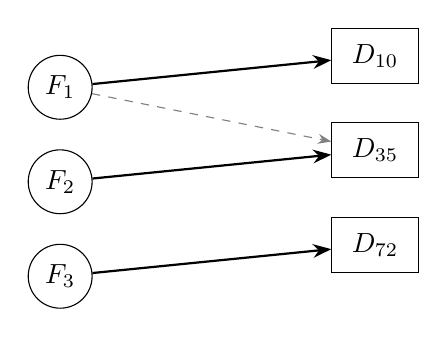
\begin{tikzpicture}[
family/.style={circle, draw, minimum size=7mm},
day/.style={rectangle, draw, minimum width=11mm, minimum height=7mm},
sel/.style={-Stealth, thick},
cand/.style={-Stealth, dashed, gray}
]
\node[family] (F1) at (0,1.2) {$F_1$};
\node[family] (F2) at (0,0) {$F_2$};
\node[family] (F3) at (0,-1.2) {$F_3$};
\node[day] (D10) at (4,1.6) {$D_{10}$};
\node[day] (D35) at (4,0.4) {$D_{35}$};
\node[day] (D72) at (4,-0.8) {$D_{72}$};
\draw[cand] (F1) -- (D35);
\draw[sel] (F1) -- (D10);
\draw[sel] (F2) -- (D35);
\draw[sel] (F3) -- (D72);
\end{tikzpicture}
\end{adjustbox}
\end{center}
\end{frame}

\begin{frame}{4. Simulated Annealing (SA)}
\textbf{Approach:}
\begin{itemize}
    \item \textbf{Neighborhood:} Randomly reassign one family to a different day from its preference list.
    \item \textbf{Efficiency:} $O(1)$ delta-cost computation by only updating affected days.
\end{itemize}

\textbf{Implementation Details:}
\begin{itemize}
    \item \textbf{Acceptance:} $P = e^{-\Delta / T}$ allows escaping local minima during high-temperature exploration.
    \item \textbf{Performance:} Reached the best overall score in our tests due to fast iterations.
\end{itemize}
\end{frame}

\begin{frame}{5. Variable Neighborhood Search (VNS)}
\textbf{Shaking Neighborhoods ($k_{max}=4$):}
\begin{enumerate}
    \item \textbf{Single Move:} Random family to random preferred day.
    \item \textbf{Swap:} Exchange days between two random families.
    \item \textbf{Chain Move:} Move family A to B's day, then B to a new day.
    \item \textbf{Redistribute:} Reassign families from a high-occupancy day.
\end{enumerate}

\textbf{Behavior:}
\begin{itemize}
    \item Uses a first-improvement local search strategy.
    \item Effective at escaping local optima but slower than SA due to full-score evaluations.
\end{itemize}
\end{frame}

\begin{frame}{6. Genetic Algorithm (GA)}
\textbf{Operators:}
\begin{itemize}
    \item \textbf{Crossover:} 50\% chance to inherit day from either parent, with feasibility checks.
    \item \textbf{Mutation:} Swap days of two random families if occupancy limits allow.
\end{itemize}

\textbf{Challenges:}
\begin{itemize}
    \item High sensitivity: small assignment changes cause large score fluctuations.
    \item Required large populations (up to 500) and generations (2000) to become competitive.
\end{itemize}
\end{frame}

\begin{frame}{7. Experimental Results: Comparative Performance}
\begin{table}[]
\centering
\small
\begin{tabular}{@{}lrrrr@{}}
\toprule
\textbf{Algorithm} & \textbf{Final Cost} & \textbf{Improvement} & \textbf{Runtime (s)} & \textbf{Stability} \\ \midrule
Simulated Annealing & \textbf{210,454} & 98.02\% & 22 & High \\
VNS & 492,944 & 95.36\% & 220 & High \\
Genetic Algorithm & 5,529,690 & 48.03\% & 338 & Low \\ \bottomrule
\end{tabular}
\caption{Best results obtained for each algorithm. Initial cost: 10,641,498.}
\end{table}
\end{frame}

\begin{frame}{8. Performance Trends}
\begin{center}
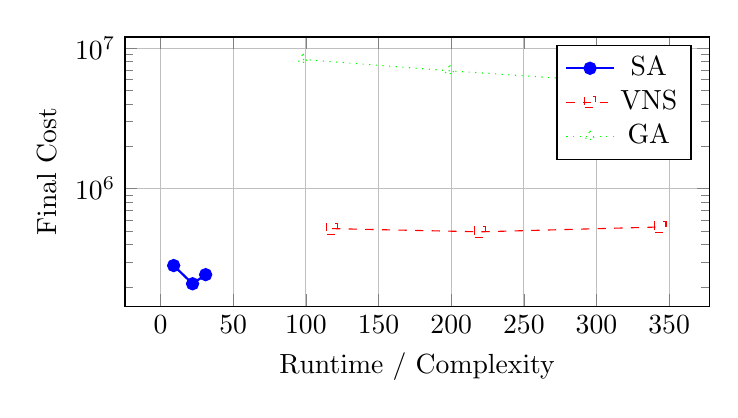
\begin{tikzpicture}
\begin{axis}[
    width=9cm, height=5cm,
    xlabel=Runtime / Complexity,
    ylabel=Final Cost,
    legend pos=north east,
    grid=major,
    ymode=log
]
% SA Best Run
\addplot[blue, thick, mark=*] coordinates { (9, 283731) (22, 210454) (31, 244355) };
\addlegendentry{SA}
% VNS Runs
\addplot[red, dashed, mark=square] coordinates { (118, 519700) (220, 492944) (344, 533905) };
\addlegendentry{VNS}
% GA Runs
\addplot[green, dotted, mark=triangle] coordinates { (98, 8307010) (199, 6896436) (338, 5529690) };
\addlegendentry{GA}
\end{axis}
\end{tikzpicture}
\end{center}
\textit{SA converges faster and to lower costs than VNS and GA in the tested scenarios.}
\end{frame}

\begin{frame}{9. Conclusions}
\begin{itemize}
    \item \textbf{SA is the superior choice:} Its ability to compute delta-costs in $O(1)$ allows for millions of iterations, exploring the state space more effectively.
    \item \textbf{VNS as a robust alternative:} While slower, the varied neighborhoods (Swaps, Chains) are effective at jumping out of local optima.
    \item \textbf{GA limitations:} The complex constraints and cost sensitivity make standard genetic operators less efficient for this specific problem.
    \item \textbf{Future Work:} Implementation of a hybrid VNS-SA approach to combine diverse neighborhoods with probabilistic acceptance.
\end{itemize}
\end{frame}

\begin{frame}{10. References \& Materials}
\textbf{Libraries \& Tools:}
\begin{itemize}
    \item \textbf{Python 3.12, Pandas, NumPy:} Used for core logic and vectorized cost calculations.
    \item \textbf{Matplotlib:} Data visualization.
\end{itemize}

\textbf{References:}
\begin{itemize}
    \item Kaggle Santa Workshop 2019: Competition documentation and forum.
    \item Gendreau, M. \& Potvin, J.-Y. \textit{Handbook of Metaheuristics}.
    \item Simulated Annealing Tutorial: "Streamlining Scheduling" (YouTube).
\end{itemize}
\end{frame}

\end{document}